\documentclass[11pt]{article}
\usepackage{fancyvrb,amsmath,amsfonts,amssymb,graphicx,parskip,listings}
\usepackage[usenames,dvipsnames,svgnames,table]{xcolor}
\usepackage{tikz}

% change margins
\addtolength{\oddsidemargin}{-.875in}
\addtolength{\evensidemargin}{-.875in}
\addtolength{\textwidth}{1.75in}
\addtolength{\topmargin}{-.875in}
\addtolength{\textheight}{1.75in}

\hyphenpenalty=10000

\begin{document}

\begin{center}
{\LARGE Eigenmath Manual}

George Weigt

December 19, 2019
\end{center}

\tableofcontents

\newpage


\section{Introduction}
The field at the bottom of the Eigenmath window is for entering
calculations that get evaluated right away.

\begin{center}
\begin{tikzpicture}
\node at (0,0) {\includegraphics[scale=0.2]{face.png}};
\draw[red,thick] (2.3,-1.85) ellipse (2.5cm and 0.5cm);
\end{tikzpicture}
\end{center}

For example, let us check the following
arithmetic from Vladimir Nabokov's autobiography {\it Speak, Memory.}

\begin{quote}
A foolish tutor had explained logarithms to me much too early, and I had
read (in a British publication, the {\it Boy's Own Paper}, I believe)
about a certain Hindu calculator who in exactly two seconds could find the
seventeenth root of, say,
%$3529471145760275132\\301897342055866171392$
% Use math mode so htlatex does not break the number
3529471145760275132301897342\\055866171392
(I am not sure I have got this right; anyway the root was 212).
\end{quote}

We can check Nabokov's arithmetic by entering the following calculation.

\begin{Verbatim}[formatcom=\color{blue}]
212^17
\end{Verbatim}

After pressing the return key, Eigenmath displays the following result.

$3529471145760275132301897342055866171392$

So Nabokov did get it right after all.
Now let us see if Eigenmath can find the
seventeenth root of this number, like the Hindu calculator could.

\begin{Verbatim}[formatcom=\color{blue}]
N = 212^17
N^(1/17)
\end{Verbatim}

Eigenmath displays the following result.

$212$

When a symbol is assigned a value, such as $N$ above,
no result is printed.
To see the value of a symbol, just evaluate it.

\begin{Verbatim}[formatcom=\color{blue}]
N
\end{Verbatim}

$N=3529471145760275132301897342055866171392$

The previous example shows a convention that will be used throughout
this manual.
That is, the color blue indicates something that the user should type.
The computer response is shown in black.


\subsection{Arithmetic}

\noindent
Normally Eigenmath uses integer and rational number arithmetic.

\begin{Verbatim}[formatcom=\color{blue}]
1/2+1/3
\end{Verbatim}

\noindent
$\displaystyle \tfrac{5}{6}$

\bigskip
\noindent
A floating point value causes Eigenmath to switch to floating point arithmetic.

\begin{Verbatim}[formatcom=\color{blue}]
1/2 + 1/3.0
\end{Verbatim}

\noindent
$\displaystyle 0.833333$

\bigskip
\noindent
An integer or rational number result can be converted to a floating
point value by entering {\it float}.

\begin{Verbatim}[formatcom=\color{blue}]
212^17
\end{Verbatim}

\noindent
$\displaystyle 3529471145760275132301897342055866171392$

\begin{Verbatim}[formatcom=\color{blue}]
float
\end{Verbatim}

\noindent
$\displaystyle 3.52947\times10^{39}$

\bigskip
\noindent
The following example shows how to enter a floating point value
using scientific notation.

\begin{Verbatim}[formatcom=\color{blue}]
epsilon = 1.0 10^(-6)
epsilon
\end{Verbatim}

\noindent
$\displaystyle \varepsilon=1.0\times10^{-6}$


\subsection{Exponents}

Eigenmath requires parentheses around negative exponents.
For example,

\begin{Verbatim}[formatcom=\color{blue}]
10^(-3)
\end{Verbatim}

\noindent
instead of

\begin{Verbatim}[formatcom=\color{blue}]
10^-3
\end{Verbatim}

\noindent
The reason for this is that the binding of the negative sign is not always
obvious.
For example, consider

\begin{Verbatim}[formatcom=\color{blue}]
x^-1/2
\end{Verbatim}

\noindent
It is not clear whether the exponent should be $-1$ or $-1/2$.
So Eigenmath requires

\begin{Verbatim}[formatcom=\color{blue}]
x^(-1/2)
\end{Verbatim}

\noindent
which is unambiguous.

\bigskip
\noindent
In general, parentheses are always required when the exponent
is an expression.
For example, \verb$x^1/2$ is evaluated as $(x^1)/2$ which
is probably not the desired result.

\begin{Verbatim}[formatcom=\color{blue}]
x^1/2
\end{Verbatim}

\noindent
$\displaystyle \tfrac{1}{2}x$

\bigskip
\noindent
Using \verb$x^(1/2)$ yields the desired result.

\begin{Verbatim}[formatcom=\color{blue}]
x^(1/2)
\end{Verbatim}

\noindent
$\displaystyle x^{1/2}$



\subsection{Symbols}
As we saw earlier, symbols are defined using an equals sign.

\begin{Verbatim}[formatcom=\color{blue}]
N = 212^17
\end{Verbatim}

No result is printed when a symbol is defined.
To see the value of a symbol, just evaluate it.

\begin{Verbatim}[formatcom=\color{blue}]
N
\end{Verbatim}

$\displaystyle N=3529471145760275132301897342055866171392$

Symbols can have more that one letter.
Everything after the first letter is displayed as a subscript.

\begin{Verbatim}[formatcom=\color{blue}]
NA = 6.02214*10^23
NA
\end{Verbatim}

$\displaystyle N_A=6.02214\times10^{23}$

A symbol can be the name of a Greek letter.

\begin{Verbatim}[formatcom=\color{blue}]
xi = 1/2
xi
\end{Verbatim}

$\displaystyle \xi=\frac{1}{2}$

Greek letters can appear in subscripts.

\begin{Verbatim}[formatcom=\color{blue}]
Amu = 2.0
Amu
\end{Verbatim}

$\displaystyle A_\mu=2.0$

The following example shows how
Eigenmath scans the entire symbol to find Greek letters.

\begin{Verbatim}[formatcom=\color{blue}]
alphamunu = 1
alphamunu
\end{Verbatim}

$\displaystyle \alpha_{\mu\nu}=1$

When a symbolic chain is defined,
Eigenmath follows the chain as far as possible.
The following example sets $A=B$ followed by $B=C$.
Then when $A$ is evaluated, the result is $C$.

\begin{Verbatim}[formatcom=\color{blue}]
A = B
B = C
A
\end{Verbatim}

$\displaystyle A=C$

Although $A=C$ is printed,
inside the program the binding of $A$ is still $B$, as can be seen with
the $binding$ function.

\begin{Verbatim}[formatcom=\color{blue}]
binding(A)
\end{Verbatim}

$\displaystyle B$

The {\it quote} function returns its argument unevaluated
and can be used to clear a symbol.
The following example clears $A$ so that its evaluation goes back to
being $A$ instead of $C$.

\begin{Verbatim}[formatcom=\color{blue}]
A = quote(A)
A
\end{Verbatim}

$\displaystyle A$

\subsection{User-defined functions}
The following example shows
a user-defined function with a single argument.

\begin{Verbatim}[formatcom=\color{blue}]
f(x) = sin(x)/x
f(pi/2)
\end{Verbatim}

$\displaystyle \frac{2}{\pi}$

The following example defines a function with two arguments.

\begin{Verbatim}[formatcom=\color{blue}]
g(x,y) = abs(x) + abs(y)
g(1,-2)
\end{Verbatim}

$\displaystyle 3$

User-defined functions can be evaluated without an argument list.
The binding of the function name is returned when there is no
argument list.

\begin{Verbatim}[formatcom=\color{blue}]
f(x) = sin(x)/x
f
\end{Verbatim}

$\displaystyle f=\frac{\sin(x)}{x}$

Normally a function body is not evaluated when a function is defined.
However, in some cases it is required that the function body be the
result of something.
The $eval$ function is used to accomplish this.
For example, the following code causes the function body to be a sixth order Taylor series expansion of $\cos x$.

\begin{Verbatim}[formatcom=\color{blue}]
f(x) = eval(taylor(cos(x),x,6))
f
\end{Verbatim}

$\displaystyle f=-\frac{1}{720}x^6+\frac{1}{24}x^4-\frac{1}{2}x^2+1$



\subsection{Scripts}
Scripting is a way of automatically running a sequence of calculations.
A script is entered in the left-hand field of the Eigenmath window.

\begin{center}
\begin{tikzpicture}
\node at (0,0) {\includegraphics[scale=0.2]{face.png}};
\draw (-2.4,0.1) node {Scripts go here.};
\end{tikzpicture}
\end{center}

To create a script, enter one calculation per line in the script field.
Nothing happens until the Run button is clicked. When the Run button is
clicked, Eigenmath evaluates the script line by line. After a script runs,
all of its symbols are available for immediate mode calculation.
Scripts can be saved and loaded using the File menu.

Here is an example script that can be pasted into the script field
and then run by clicking the Run button.

\begin{Verbatim}[formatcom=\color{blue}]
"Solve for vector X in AX = B"
A = ((1,2),(3,4))
B = (5,6)
X = dot(inv(A),B)
X
\end{Verbatim}

After clicking the Run button, the following result is displayed.

\verb$Solve for vector X in AX = B$

$\displaystyle X=\begin{bmatrix}-4\\ \frac{9}{2}\end{bmatrix}$

A handy debugging aid is to include the line $trace=1$ in the script.
When $trace=1$ each line of the script is displayed as it is evaluated.
For example, here is the previous script with the addition of
$trace=1$.

\begin{Verbatim}[formatcom=\color{blue},samepage=true]
"Solve for vector X in AX = B"
trace = 1
A = ((1,2),(3,4))
B = (5,6)
X = dot(inv(A),B)
X
\end{Verbatim}

The result is

\begin{Verbatim}
Solve for vector X in AX = B
A = ((1,2),(3,4))
B = (5,6)
X = dot(inv(A),B)
X
\end{Verbatim}

$X=\begin{bmatrix}-4\\ \frac{9}{2}\end{bmatrix}$


\subsection{Draw}

$draw(f,x)$ draws a graph of the function $f$ of $x$.
The second argument can be omitted when the dependent variable
is literally $x$ or $t$.
The vectors $xrange$ and $yrange$ control the scale of the graph.

{\color{blue}
\begin{verbatim}
draw(x^2)
\end{verbatim}
}

\begin{center}
\includegraphics[scale=0.2]{parabola.png}
\end{center}

{\color{blue}
\begin{verbatim}
xrange = (-1,1)
yrange = (0,2)
draw(x^2)
\end{verbatim}
}

\begin{center}
\includegraphics[scale=0.2]{parabola2.png}
\end{center}

\noindent
Parametric drawing occurs when a function returns a vector.
The vector $trange$ controls the parametric range.
The default is $trange=(-\pi,\pi)$.
In the following example, $draw$ varies $theta$
over the default range $-\pi$ to $+\pi$.

{\color{blue}
\begin{verbatim}
xrange = (-10,10)
yrange = (-10,10)
f = (cos(theta),sin(theta))
draw(5 f,theta)
\end{verbatim}
}

\begin{center}
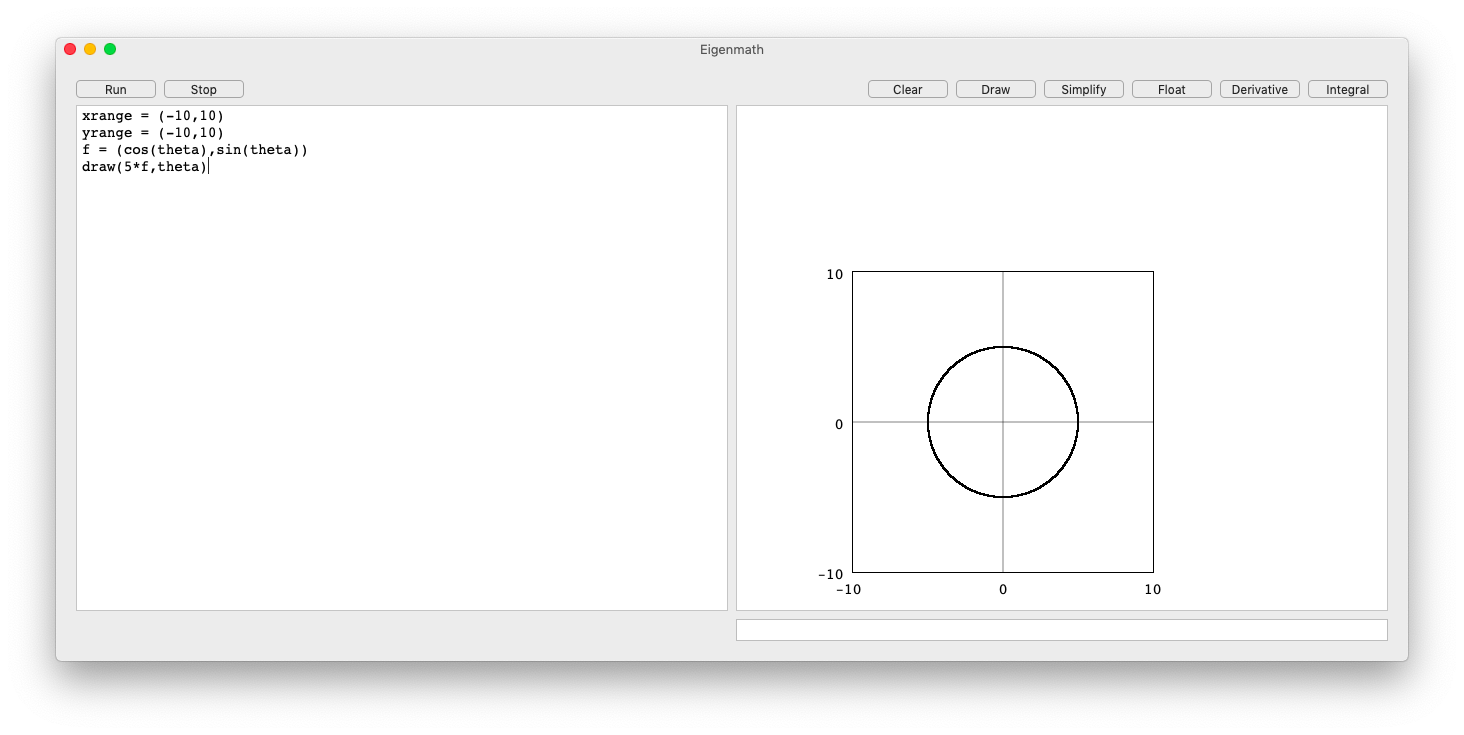
\includegraphics[scale=0.2]{circle.png}
\end{center}

\noindent
In the following example, $trange$ is reduced
to draw a quarter circle instead of a full circle.

{\color{blue}
\begin{verbatim}
trange = (0,pi/2)
f = (cos(theta),sin(theta))
draw(5 f,theta)
\end{verbatim}
}

\begin{center}
\includegraphics[scale=0.2]{circle2.png}
\end{center}

\noindent
Here are a couple of interesting curves and the code for drawing them.
First is a lemniscate.

{\color{blue}
\begin{verbatim}
trange = (-pi,pi)
X = cos(t)/(1 + sin(t)^2)
Y = sin(t) cos(t)/(1 + sin(t)^2)
f = (X,Y)
draw(5 f,t)
\end{verbatim}
}

\begin{center}
\includegraphics[scale=0.2]{lemniscate.png}
\end{center}

\noindent
Next is a cardioid.

{\color{blue}
\begin{verbatim}
r = (1 + cos(t))/2
u = (cos(t),sin(t))
xrange = (-1,1)
yrange = (-1,1)
trange = (0,2 pi)
draw(r u,t)
\end{verbatim}
}

\begin{center}
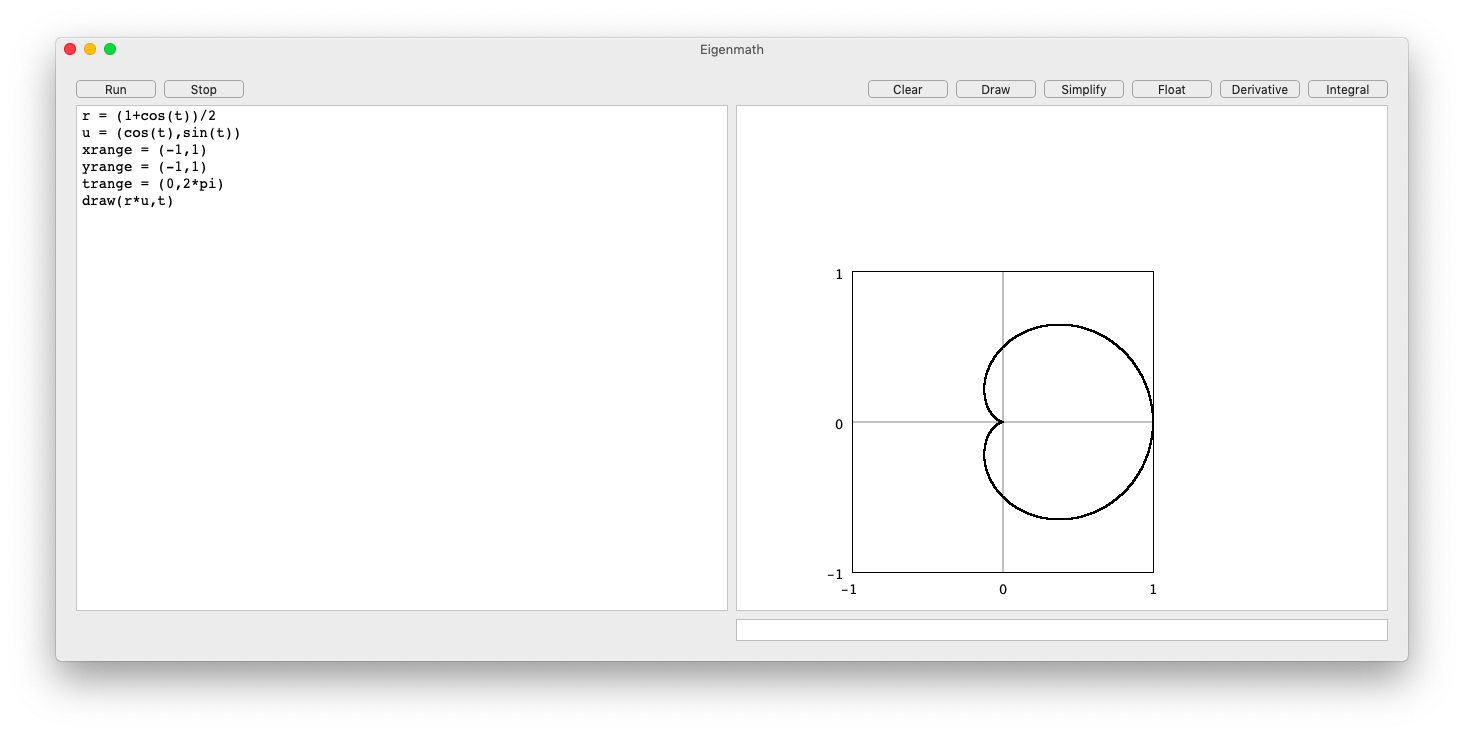
\includegraphics[scale=0.2]{cardioid.png}
\end{center}


\subsection{Complex numbers}

When Eigenmath starts up, it defines symbol $i$ as $i=\sqrt{-1}$.
Symbol $i$ can be redefined and used for some other purpose if need be.

\bigskip
\noindent
Complex quantities can be entered in either rectangular or polar form.

{\color{blue}
\begin{verbatim}
a + i b
\end{verbatim}
}

\noindent
$a+ib$

{\color{blue}
\begin{verbatim}
exp(1/3 i pi)
\end{verbatim}
}

\noindent
$\exp\left(\tfrac{1}{3}i\pi\right)$

\bigskip
\noindent
Converting a complex number to rectangular or polar coordinates causes
simplification of mixed forms.

{\color{blue}
\begin{verbatim}
A = 1 + i
B = sqrt(2) exp(1/4 i pi)
A - B
\end{verbatim}
}

\noindent
$1+i-2^{1/2}\exp\left(\tfrac{1}{4}i\pi\right)$

{\color{blue}
\begin{verbatim}
rect(last)
\end{verbatim}
}

\noindent
$0$

\bigskip
\noindent
Rectangular complex quantities, when raised to a power, are multiplied out.

{\color{blue}
\begin{verbatim}
(a + i b)^2
\end{verbatim}
}

\noindent
$a^2-b^2+2iab$

\bigskip
\noindent
When $a$ and $b$ are numerical and the power is negative, the evaluation is done as follows.
\begin{equation*}
(a+ib)^{-n}
=\left(\frac{a-ib}{(a+ib)(a-ib)}\right)^n=
\left(\frac{a-ib}{a^2+b^2}\right)^n
\end{equation*}

\noindent
Here are a few examples.

{\color{blue}
\begin{verbatim}
1/(2 - i)
\end{verbatim}
}

\noindent
$\tfrac{2}{5}+\frac{1}{5}i$

{\color{blue}
\begin{verbatim}
(-1 + 3 i)/(2 - i)
\end{verbatim}
}

\noindent
$-1+i$

\bigskip
\noindent
The absolute value of a complex number returns its magnitude.

{\color{blue}
\begin{verbatim}
abs(3 + 4 i)
\end{verbatim}
}

\noindent
$5$

\bigskip
\noindent
Since symbols can have complex values, the absolute value
of a symbolic expression is not computed.

{\color{blue}
\begin{verbatim}
abs(a + b i)
\end{verbatim}
}

\noindent
$\operatorname{abs}(a+ib)$

\bigskip
\noindent
The $mag$ function can be used instead of $abs$.
It treats symbols like $a$ and $b$ as real.

{\color{blue}
\begin{verbatim}
mag(a + b i)
\end{verbatim}
}

\noindent
$\displaystyle (a^2+b^2)^{1/2}$

\bigskip
\noindent
The imaginary unit can be changed from $i$ to $j$
by defining $j=\sqrt{-1}$.

{\color{blue}
\begin{verbatim}
j = sqrt(-1)
sqrt(-4)
\end{verbatim}
}

\noindent
$\displaystyle 2j$


\subsection{Linear algebra}

The $dot$ function is used to multiply tensors.
For example, let
\begin{equation*}
A=\begin{pmatrix}1&2\\3&4\end{pmatrix}
\quad{\rm and}\quad x=\begin{pmatrix}x_1\\x_2\end{pmatrix}
\end{equation*}

\noindent
The product $Ax$ is computed as follows.

{\color{blue}
\begin{verbatim}
A = ((1,2),(3,4))
x = (x1,x2)
dot(A,x)
\end{verbatim}
}

\noindent
$\begin{bmatrix}
x_1+2x_2\\
3x_1+4x_2
\end{bmatrix}$

\bigskip
\noindent
The following example shows how to use $dot$ and $inv$ to solve for
the vector $X$ in $AX=B$.

{\color{blue}
\begin{verbatim}
A = ((3,7),(1,-9))
B = (16,-22)
X = dot(inv(A),B)
X
\end{verbatim}
}

\noindent
$X=\begin{bmatrix}-\tfrac{5}{17}\\ \\ \tfrac{41}{17}\end{bmatrix}$

\bigskip
\noindent
The $dot$ function can have more than two arguments.
For example, $dot(A,B,C)$ can be used for the dot product of three tensors.

\bigskip
\noindent
Square brackets are used for component access.
Index numbering starts with 1.

{\color{blue}
\begin{verbatim}
A = ((a,b),(c,d))
A[1,2] = -A[1,1]
A
\end{verbatim}
}

\noindent
$\begin{bmatrix}a&-a\\c&d\end{bmatrix}$

\bigskip
\noindent
The following example demonstrates the relation
$A^{-1}=\frac{\operatorname{adj}A}{\operatorname{det}A}$.

{\color{blue}
\begin{verbatim}
A = ((a,b),(c,d))
inv(A)
\end{verbatim}
}

\noindent
$\begin{bmatrix}\frac{d}{ad-bc} & -\frac{b}{ad-bc}\\-\frac{c}{ad-bc} & \frac{a}{ad-bc}\end{bmatrix}$

{\color{blue}
\begin{verbatim}
adj(A)
\end{verbatim}
}

\noindent
$\begin{bmatrix}d & -b\\-c & a\end{bmatrix}$

{\color{blue}
\begin{verbatim}
det(A)
\end{verbatim}
}

\noindent
$ad-bc$

{\color{blue}
\begin{verbatim}
inv(A) - adj(A)/det(A)
\end{verbatim}
}

\noindent
$\begin{bmatrix}0 & 0\\0 & 0\end{bmatrix}$

\bigskip
\noindent
Sometimes a calculation will be simpler if it can be reorganized to use
$adj$ instead of $inv$.
The main idea is to try to prevent the determinant from appearing as a
divisor.
For example, suppose for matrices $A$ and $B$ you want to check that
\begin{equation*}
{A}-{B}^{-1}=0
\end{equation*}
Depending on the complexity of $\mathop{\rm det}B$, the software
may not be able to find a simplification that yields zero.
Should that occur, the following alternative formulation can be tried.
\begin{equation*}
A\operatorname{det}B-\operatorname{adj}B=0
\end{equation*}


\section{Calculus}

\subsection{Derivative}

$d(f,x)$ returns the derivative of $f$ with respect to $x$.
The $x$ can be omitted for expressions in $x$.

{\color{blue}
\begin{verbatim}
d(x^2)
\end{verbatim}
}

\noindent
$2x$

\bigskip
\noindent
The following table summarizes the various ways to obtain multi-derivatives.

\begin{center}
\begin{tabular}{cllllll}
$\displaystyle{\frac{\partial^2f}{\partial x^2}}$ & & \verb$d(f,x,x)$ & & \verb$d(f,x,2)$ \\
\\
$\displaystyle{\frac{\partial^2f}{\partial x\,\partial y}}$ & & \verb$d(f,x,y)$ \\
\\
$\displaystyle{\frac{\partial^{m+n+\cdot\cdot\cdot} f}{\partial x^m\,\partial y^n\cdots}}$ & &
\verb$d(f,x,...,y,...)$ & & \verb$d(f,x,m,y,n,...)$ \\
\end{tabular}
\end{center}

\subsection{Gradient}

The gradient of $f$ is obtained by using a vector for $x$ in $d(f,x)$.

{\color{blue}
\begin{verbatim}
r = sqrt(x^2 + y^2)
d(r,(x,y))
\end{verbatim}
}

\noindent
$\begin{bmatrix}\frac{x}{(x^2+y^2)^{1/2}}\\ \frac{y}{(x^2+y^2)^{1/2}}\end{bmatrix}$

\bigskip
\noindent
The $f$ in $d(f,x)$ can be a tensor function.
Gradient raises the rank by one.

{\color{blue}
\begin{verbatim}
F = (x + 2 y,3 x + 4 y)
X = (x,y)
d(F,X)
\end{verbatim}
}

\noindent
$\begin{bmatrix}1&2\\3&4\end{bmatrix}$

\subsection{Template functions}

The function $f$ in $d(f)$ does not have to be defined.
It can be a template function with just a name and an argument list.
Eigenmath checks the argument list to figure out what to do.
For example, $d(f(x),x)$ evaluates to itself because $f$ depends on $x$.
However, $d(f(x),y)$ evaluates to zero because $f$ does not depend on $y$.

{\color{blue}
\begin{verbatim}
d(f(x),x)
\end{verbatim}
}

\noindent
$\operatorname{d}(f(x),x)$

{\color{blue}
\begin{verbatim}
d(f(x),y)
\end{verbatim}
}

\noindent
$0$

{\color{blue}
\begin{verbatim}
d(f(x,y),y)
\end{verbatim}
}

\noindent
$\operatorname{d}(f(x,y),y)$

{\color{blue}
\begin{verbatim}
d(f(),t)
\end{verbatim}
}

\noindent
$\operatorname{d}(f(),t)$

\bigskip
\noindent
As the final example shows, an empty argument list causes
$d(f)$ to always evaluate to itself, regardless
of the second argument.

\bigskip
\noindent
Template functions are useful for experimenting with differential forms.
For example, let us check the identity
$$\operatorname{div}(\operatorname{curl}{F})=0$$
for an arbitrary vector function $F$.

{\color{blue}
\begin{verbatim}
F = (F1(x,y,z),F2(x,y,z),F3(x,y,z))
curl(U) = (d(U[3],y) - d(U[2],z),d(U[1],z) - d(U[3],x),d(U[2],x) - d(U[1],y))
div(U) = d(U[1],x) + d(U[2],y) + d(U[3],z)
div(curl(F))
\end{verbatim}
}

\noindent
$0$



\subsection{Integral}
$integral(f,x)$ returns the integral of $f$ with respect to $x$.
The $x$ can be omitted for expressions in $x$.
The argument list can be extended for multiple integrals.

\begin{Verbatim}[formatcom=\color{blue},samepage=true]
integral(x^2)
\end{Verbatim}

$\displaystyle \frac{1}{3}x^3$

\begin{Verbatim}[formatcom=\color{blue},samepage=true]
integral(x*y,x,y)
\end{Verbatim}

$\displaystyle \frac{1}{4}x^2y^2$

$defint(f,x,a,b,\ldots)$
computes the definite integral of $f$ with respect to $x$ evaluated from
$a$ to $b$.
The argument list can be extended for multiple integrals.
The following example computes the integral of $f=x^2$
over the domain of a semicircle.
For each $x$ along the abscissa, $y$ ranges from 0 to $\sqrt{1-x^2}$.

\begin{Verbatim}[formatcom=\color{blue},samepage=true]
defint(x^2,y,0,sqrt(1-x^2),x,-1,1)
\end{Verbatim}

$\displaystyle \frac{1}{8}\pi$

As an alternative, the $eval$ function can be used to compute a definite integral step by step.

\begin{Verbatim}[formatcom=\color{blue},samepage=true]
I = integral(x^2,y)
I = eval(I,y,sqrt(1-x^2))-eval(I,y,0)
I = integral(I,x)
eval(I,x,1)-eval(I,x,-1)
\end{Verbatim}

$\displaystyle \frac{1}{8}\pi$



\bigskip
\noindent
Here is a useful trick.
Difficult integrals involving sine and cosine
can often be solved by using exponentials.
Trigonometric simplifications involving powers
and multiple angles turn into simple algebra in the
exponential domain.
For example, the definite integral
$$\int_0^{2\pi}\left(\sin^4t-2\cos^3(t/2)\sin t\right)dt$$
can be solved as follows.

\begin{Verbatim}[formatcom=\color{blue},samepage=true]
f = sin(t)^4-2*cos(t/2)^3*sin(t)
f = circexp(f)
defint(f,t,0,2*pi)
\end{Verbatim}

\noindent
$\displaystyle -\frac{16}{5}+\frac{3}{4}\pi$

\bigskip
\noindent
Here is a check of the result.

\begin{Verbatim}[formatcom=\color{blue},samepage=true]
g = integral(f,t)
f-d(g,t)
\end{Verbatim}

\noindent
$\displaystyle 0$


The fundamental theorem of calculus
is a formal expression of the inverse relation between
integrals and derivatives.
$$\int_a^b f'(x)\,dx=f(b)-f(a)$$
Here is an Eigenmath demonstration of the fundamental theorem of calculus.

\begin{Verbatim}[formatcom=\color{blue},samepage=true]
xrange = (-1,1)
yrange = (-1,1)
f = d(x^2/2)
draw(f,x)
\end{Verbatim}

\begin{center}
\includegraphics[scale=0.2]{funda1.png}
\end{center}

\begin{Verbatim}[formatcom=\color{blue},samepage=true]
xrange = (-1,1)
yrange = (-1,1)
f = integral(d(x^2/2))
draw(f,x)
\end{Verbatim}

\begin{center}
\includegraphics[scale=0.2]{funda2.png}
\end{center}

The first graph shows that $f'(x)$ is antisymmetric, therefore the total
area under the curve from $-1$ to $1$ sums to zero.
The second graph shows that $f(1)=f(-1)$.
Hence for $f(x)={1\over2}x^2$ we have
$$\int_{-1}^1f'(x)\,dx=f(1)-f(-1)=0$$


\subsection{Arc length}

Let $g(t)$ be a function that draws a curve.
The arc length from $g(a)$ to $g(b)$ is given by
$$\int_a^b|g'(t)|\,dt$$
where $|g'(t)|$ is the length of the tangent vector at $g(t)$.
The integral sums over all of the tangent lengths to arrive at the total length
from $a$ to $b$.
For example, let us measure the length of the following curve.

{\color{blue}
\begin{verbatim}
xrange = (0,1)
yrange = (0,1)
draw(x^2)
\end{verbatim}
}

\begin{center}
\includegraphics[scale=0.2]{arc.png}
\end{center}

\noindent
A suitable $g(t)$ for the arc is
$$g(t)=(t,t^2),\quad0\le t\le1$$
Hence one Eigenmath solution for computing the arc length is

\begin{Verbatim}[formatcom=\color{blue},samepage=true]
x = t
y = t^2
g = (x,y)
defint(abs(d(g,t)),t,0,1)
\end{Verbatim}

\noindent
$\displaystyle \frac{1}{4}\log(2+5^{1/2})+\frac{1}{2}5^{1/2}$

\begin{Verbatim}[formatcom=\color{blue},samepage=true]
float
\end{Verbatim}

\noindent
$\displaystyle 1.47894$

\bigskip
\noindent
As expected, the result is greater than $\sqrt2\approx1.414$,
the length of the
diagonal from $(0,0)$ to $(1,1)$.

\bigskip
\noindent
The result seems rather complicated given that we
started with a simple parabola.
Let us inspect $|g'(t)|$ to see why.

\begin{Verbatim}[formatcom=\color{blue},samepage=true]
g
\end{Verbatim}

\noindent
$\displaystyle g=\begin{bmatrix}t\\ t^2\end{bmatrix}$

\begin{Verbatim}[formatcom=\color{blue},samepage=true]
d(g,t)
\end{Verbatim}

\noindent
$\displaystyle \begin{bmatrix}1\\ 2t\end{bmatrix}$

\begin{Verbatim}[formatcom=\color{blue},samepage=true]
abs(d(g,t))
\end{Verbatim}

\noindent
$\displaystyle (4t^2+1)^{1/2}$

\bigskip
\noindent
The following script does a discrete computation of the arc length
by dividing the curve into 100 pieces.

\begin{Verbatim}[formatcom=\color{blue},samepage=true]
g(t) = (t,t^2)
h(k) = abs(g(k/100.0) - g((k-1)/100.0))
sum(k,1,100,h(k))
\end{Verbatim}

\noindent
$\displaystyle 1.47894$

\bigskip
\noindent
As expected, the discrete result matches the analytic result.

\bigskip
\noindent
Find the length of the curve $y=x^{3/2}$ from the origin to
$x={4\over3}$.

\begin{Verbatim}[formatcom=\color{blue},samepage=true]
x = t
y = x^(3/2)
g = (x,y)
defint(abs(d(g,x)),x,0,4/3)
\end{Verbatim}

\noindent
$\displaystyle \frac{56}{27}$

\bigskip
\noindent
Because of the way $t$ is substituted for $x$,
the following code yields the same result.

\begin{Verbatim}[formatcom=\color{blue},samepage=true]
g = (t,t^(3/2))
defint(abs(d(g,t)),t,0,4/3)
\end{Verbatim}

\noindent
$\displaystyle \frac{56}{27}$

\subsection{Line integrals}
There are two different kinds of line integrals,
one for scalar fields and one
for vector fields.
The following table shows how both are based on the calculation of
arc length.

\begin{center}
\begin{tabular}{|l|l|l|}
\hline
& Abstract form
& Computable form
\\
\hline
 & &\\
Arc length
& $\displaystyle{\int_C ds}$
& $\displaystyle{\int_a^b |g'(t)|\,dt}$\\
 & &\\
\hline
 & & \\
Line integral, scalar field
& $\displaystyle{\int_C f\,ds}$
& $\displaystyle{\int_a^b f(g(t))\,|g'(t)|\,dt}$\\
& &\\
\hline
 & & \\
Line integral, vector field
& $\displaystyle{\int_C(F\cdot u)\,ds}$
& $\displaystyle{\int_a^b F(g(t))\cdot g'(t)\,dt}$\\
 & & \\
\hline
\end{tabular}
\end{center}

\noindent
For the vector field form, the symbol $u$ is the unit tangent vector
$$u={g'(t)\over|g'(t)|}$$
The length of the tangent vector cancels with $ds$
as follows.
$$\int_C(F\cdot u)\,ds
=\int_a^b\bigg(F(g(t))\cdot{g'(t)\over|g'(t)|}\bigg)\,\bigg(|g'(t)|\,dt\bigg)
=\int_a^b F(g(t))\cdot g'(t)\,dt
$$

\noindent
Evaluate
$$\int_Cx\,ds\quad\hbox{and}\quad\int_Cx\,dx$$
where $C$ is a straight line from $(0,0)$ to $(1,1)$.

\bigskip
\noindent
What a difference the measure makes.
The first integral is over a scalar field and the second is over a vector field.
This can be understood when we recall that
$$ds=|g'(t)|\,dt
%\quad\hbox{and}\quad
%\int_Cx\,dx=\int_Cx\,dx+0\,dy
$$
Hence for $\int_Cx\,ds$ we have

\begin{Verbatim}[formatcom=\color{blue},samepage=true]
x = t
y = t
g = (x,y)
defint(x*abs(d(g,t)),t,0,1)
\end{Verbatim}

\noindent
$\displaystyle \frac{1}{2^{1/2}}$

\bigskip
\noindent
For $\int_Cx\,dx$ we have

\begin{Verbatim}[formatcom=\color{blue},samepage=true]
x = t
y = t
g = (x,y)
F = (x,0)
defint(dot(F,d(g,t)),t,0,1)
\end{Verbatim}

\noindent
$\displaystyle \frac{1}{2}$

\bigskip
\noindent
The following line integral problems are from
{\it Advanced Calculus, Fifth Edition} by Wilfred Kaplan.

\bigskip
\noindent
Evaluate $\int y^2\,dx$ along the straight
line from $(0,0)$ to $(2,2)$.

\begin{Verbatim}[formatcom=\color{blue},samepage=true]
x = 2t
y = 2t
g = (x,y)
F = (y^2,0)
defint(dot(F,d(g,t)),t,0,1)
\end{Verbatim}

\noindent
$\displaystyle \frac{8}{3}$

\bigskip
\noindent
Evaluate $\int z\,dx+x\,dy+y\,dz$
along the path
$x=2t+1$, $y=t^2$, $z=1+t^3$, $0\le t\le 1$.

\begin{Verbatim}[formatcom=\color{blue},samepage=true]
x = 2t+1
y = t^2
z = 1+t^3
g = (x,y,z)
F = (z,x,y)
defint(dot(F,d(g,t)),t,0,1)
\end{Verbatim}

\noindent
$\displaystyle \frac{163}{30}$



\subsection{Surface area}
Let $S$ be a surface parameterized by $x$ and $y$.
That is, let $S=(x,y,z)$ where $z=f(x,y)$.
The tangent lines at a point on $S$ form a tiny parallelogram.
The area $a$ of the parallelogram is given by the magnitude of the cross product.
$$a=\left|\frac{\partial S}{\partial x}\times\frac{\partial S}{\partial y}\right|$$
By summing over all the parallelograms we obtain the total surface area $A$.
Hence
$$A=\int\!\!\!\int dA=\int\!\!\!\int a\,dx\,dy$$
The following example computes the surface area of a unit disk
parallel to the $xy$ plane.

\begin{Verbatim}[formatcom=\color{blue},samepage=true]
z = 2
S = (x,y,z)
a = abs(cross(d(S,x),d(S,y)))
defint(a,y,-sqrt(1 - x^2),sqrt(1 - x^2),x,-1,1)
\end{Verbatim}

\noindent
$\displaystyle \pi$

\bigskip
\noindent
The result is $\pi$, the area of a unit circle, which is what we expect.
The following example computes the surface area of $z=x^2+2y$ over
a unit square.

\begin{Verbatim}[formatcom=\color{blue},samepage=true]
z = x^2 + 2y
S = (x,y,z)
a = abs(cross(d(S,x),d(S,y)))
defint(a,x,0,1,y,0,1)
\end{Verbatim}

\noindent
$\displaystyle \tfrac{5}{8}\log(5)+\tfrac{3}{2}$

\bigskip
\noindent
The following exercise is from
{\it Multivariable Mathematics} by Williamson and Trotter, p. 598.
Find the area of the spiral ramp defined by
$$S=\begin{bmatrix}u\cos v\\\ u\sin v\\ v\end{bmatrix},\qquad 0\le u\le1,\qquad 0\le v\le3\pi$$

\begin{Verbatim}[formatcom=\color{blue},samepage=true]
x = u cos(v)
y = u sin(v)
z = v
S = (x,y,z)
a = abs(cross(d(S,u),d(S,v)))
defint(a,u,0,1,v,0,3pi)
\end{Verbatim}

\noindent
$\displaystyle \tfrac{3}{2}\pi\log(1+2^{1/2})+\frac{3\pi}{2^{1/2}}$

\begin{Verbatim}[formatcom=\color{blue},samepage=true]
float
\end{Verbatim}

\noindent
$\displaystyle 10.8177$



\subsection{Surface integrals}
A surface integral is like adding up all the wind on a sail.
In other words, we want to compute
$$\int\!\!\!\int{\bf F\cdot n}\,dA$$
where ${\bf F\cdot n}$ is the amount of wind normal to a tiny parallelogram $dA$.
The integral sums over the entire area of the sail.
Let $S$ be the surface of the sail parameterized by $x$ and $y$.
(In this model, the $z$ direction points downwind.)
By the properties of the cross product we have the following for the unit normal $\bf n$
and for $dA$.
$${\bf n}={ {{\partial S\over\partial x}\times{\partial S\over\partial y}}\over
 {\left|{\partial S\over\partial x}\times{\partial S\over\partial y}\right|}}\qquad
dA=\left|{\partial S\over\partial x}\times{\partial S\over\partial y}\right|\,dx\,dy$$
Hence
$$\int\!\!\!\int{\bf F\cdot n}\,dA=\int\!\!\!\int{\bf F}\cdot
\left({{\partial S\over\partial x}\times{\partial S\over\partial y}}\right)\,dx\,dy$$

\bigskip
\noindent
The following exercise is from
{\it Advanced Calculus} by Wilfred Kaplan, p.~313.
Evaluate the surface integral
$$\int\!\!\!\int_S{\bf F\cdot n}\,d\sigma$$

\noindent
where ${\bf F}=xy^2z{\bf i}-2x^3{\bf j}+yz^2{\bf k}$, $S$ is the surface
$z=1-x^2-y^2$, $x^2+y^2\le1$ and $\bf n$ is upper.

\bigskip
\noindent
Note that the surface intersects the $xy$ plane in a circle.
By the right hand rule, crossing $x$ into $y$ yields $\bf n$ pointing upwards hence
$${\bf n}\,d\sigma=\left({{\partial S\over\partial x}\times{\partial S\over\partial y}}\right)\,dx\,dy$$

\noindent
The following Eigenmath code computes the surface integral.
The symbols $f$ and $h$ are used as temporary variables.

\begin{Verbatim}[formatcom=\color{blue},samepage=true]
z = 1-x^2-y^2
F = (x*y^2*z,-2*x^3,y*z^2)
S = (x,y,z)
f = dot(F,cross(d(S,x),d(S,y)))
h = sqrt(1-x^2)
defint(f,y,-h,h,x,-1,1)
\end{Verbatim}

\noindent
$\displaystyle \frac{1}{48}\pi$



\subsection{Green's theorem}
Green's theorem tells us that
$$\oint P\,dx+Q\,dy=\int\!\!\!\int
\left(\frac{\partial Q}{\partial x}-\frac{\partial P}{\partial y}\right)
dx\,dy$$

\noindent
In other words, a line integral and a surface integral can yield
the same result.

\bigskip
\noindent
Example 1.
The following exercise is from {\it Advanced Calculus}
by Wilfred Kaplan, p.~287.
Evaluate $\oint (2x^3-y^3)\,dx+(x^3+y^3)\,dy$ around the circle
$x^2+y^2=1$ using Green's theorem.

\bigskip
\noindent
It turns out that Eigenmath cannot solve the double integral over
$x$ and $y$ directly.
Polar coordinates are used instead.

\begin{Verbatim}[formatcom=\color{blue},samepage=true]
P = 2x^3 - y^3
Q = x^3 + y^3
f = d(Q,x) - d(P,y)
x = r cos(theta)
y = r sin(theta)
defint(f r,r,0,1,theta,0,2pi)
\end{Verbatim}

\noindent
$\displaystyle \tfrac{3}{2}\pi$

\bigskip
\noindent
The $defint$ integrand is $f\,r$ because $r\,dr\,d\theta=dx\,dy$.

\bigskip
\noindent
Now let us try computing the line integral side of Green's theorem
and see if we get the same result.
We need to use the trick of converting sine and cosine to exponentials
so that Eigenmath can find a solution.

\begin{Verbatim}[formatcom=\color{blue},samepage=true]
x = cos(t)
y = sin(t)
P = 2x^3 - y^3
Q = x^3 + y^3
f = P d(x,t) + Q d(y,t)
f = circexp(f)
defint(f,t,0,2pi)
\end{Verbatim}

\noindent
$\displaystyle \tfrac{3}{2}\pi$

\bigskip
\noindent
Example 2.
Compute both sides of Green's theorem for
$F=(1-y,x)$ over the disk $x^2+y^2\le4$.

\bigskip
\noindent
First compute the line integral along the boundary of the disk.
Note that the radius of the disk is 2.

\begin{Verbatim}[formatcom=\color{blue},samepage=true]
-- Line integral
P = 1 - y
Q = x
x = 2 cos(t)
y = 2 sin(t)
defint(P d(x,t) + Q d(y,t),t,0,2pi)
\end{Verbatim}

\noindent
$\displaystyle 8\pi$

\begin{Verbatim}[formatcom=\color{blue},samepage=true]
-- Surface integral
x = quote(x) --clear x
y = quote(y) --clear y
h = sqrt(4-x^2)
defint(d(Q,x)-d(P,y),y,-h,h,x,-2,2)
\end{Verbatim}

\noindent
$\displaystyle 8\pi$

\begin{Verbatim}[formatcom=\color{blue},samepage=true]
-- Try computing the surface integral using polar coordinates.
f = d(Q,x) - d(P,y) --do before change of coordinates
x = r cos(theta)
y = r sin(theta)
defint(f r,r,0,2,theta,0,2pi)
\end{Verbatim}

\noindent
$\displaystyle 8\pi$

\begin{Verbatim}[formatcom=\color{blue},samepage=true]
defint(f r,theta,0,2pi,r,0,2) --try integrating over theta first
\end{Verbatim}

\noindent
$\displaystyle 8\pi$

\bigskip
\noindent
In this case, Eigenmath solved both forms of the polar integral.
However, in cases where Eigenmath fails to solve a double integral, try
changing the order of integration.


\subsection{Stokes' theorem}

Stokes' theorem says that in typical problems a surface integral can be
computed using a line integral.
(There is some fine print regarding continuity and boundary conditions.)
This is a useful theorem because usually the line integral is easier to
compute.
In rectangular coordinates the equivalence between a line integral
on the left and a surface integral on the right is
%
$$\oint P\,dx+Q\,dy+R\,dz
=\int\!\!\!\int_S(\mathop{\rm curl}{\bf F})\cdot{\bf n}\,d\sigma
$$
%
where ${\bf F}=(P,Q,R)$.
For $S$ parametrized by $x$ and $y$ we have
$${\bf n}\,d\sigma=\left(
\frac{\partial S}{\partial x}\times\frac{\partial S}{\partial y}
\right)dx\,dy$$

\noindent
Example:
Let ${\bf F}=(y,z,x)$ and let $S$ be the part of the paraboloid
$z=4-x^2-y^2$
that is above the $xy$ plane.
The perimeter of the paraboloid is the circle $x^2+y^2=2$.
The following script computes both the line and surface integrals.
It turns out that we need to use polar coordinates for the
line integral so that {\it defint} can succeed.

{\color{blue}
\begin{verbatim}
-- www.eigenmath.org/stokes-theorem.txt
"Surface integral"
z = 4 - x^2 - y^2
F = (y,z,x)
S = (x,y,z)
f = dot(curl(F),cross(d(S,x),d(S,y)))
x = r cos(theta)
y = r sin(theta)
defint(f r,r,0,2,theta,0,2pi)
"Line integral"
x = 2 cos(t)
y = 2 sin(t)
z = 4 - x^2 - y^2
P = y
Q = z
R = x
f = P d(x,t) + Q d(y,t) + R d(z,t)
f = circexp(f)
defint(f,t,0,2pi)
\end{verbatim}
}

\noindent
This is the result when the script runs.
Both the surface integral and the line integral
yield the same result.

\bigskip
\noindent
Surface integral\\
$\displaystyle -4\pi$\\
Line integral\\
$\displaystyle -4\pi$


%%%%%

\section{Examples}


\subsection{Fran\c cois Vi\`ete}
Fran\c cois Vi\`ete was the first to discover an exact formula for $\pi$.
Here is his formula.
\begin{displaymath}
{2\over\pi}={\sqrt2\over2}\times{\sqrt{2+\sqrt2}\over2}\times
{\sqrt{2+\sqrt{2+\sqrt2}}\over2}\times\cdots
\end{displaymath}
%We can flip it around and write the formula like this.
%\begin{displaymath}
%\pi=2\times{2\over\sqrt2}\times{2\over\sqrt{2+\sqrt2}}\times
%{2\over\sqrt{2+\sqrt{2+\sqrt2}}}\times\cdots
%\end{displaymath}
Let $a_0=0$ and $a_{n}=\sqrt{2+a_{n-1}}$.
Then we can write
\begin{displaymath}
{2\over\pi}={a_1\over2}\times{a_2\over2}\times
{a_3\over2}\times\cdots
\end{displaymath}
%
Solving for $\pi$ we have
\begin{displaymath}
\pi=2\times{2\over a_1}\times{2\over a_2}\times{2\over a_3}\times\cdots=2\prod_{k=1}^\infty
{2\over a_k}
\end{displaymath}
%
Let us now use Eigenmath to compute $\pi$ according to Vi\`ete's formula.
Of course, we cannot calculate all the way out to infinity, we have to stop somewhere.
It turns out that nine factors are just enough to get six digits of accuracy.

\begin{Verbatim}[formatcom=\color{blue},samepage=true]
a(n)=test(n=0,0,sqrt(2+a(n-1)))
float(2*product(k,1,9,2/a(k)))
\end{Verbatim}

$\displaystyle 3.14159$

The function $a(n)$ calls itself $n$ times so overall there are
54 calls to $a(n)$.
By using a different algorithm with temporary variables, we can get the
answer in just nine steps.

\begin{Verbatim}[formatcom=\color{blue},samepage=true]
a = 0
b = 2
for(k,1,9,a=sqrt(2+a),b=b*2/a)
float(b)
\end{Verbatim}

$\displaystyle 3.14159$



\subsection{Curl in tensor form}
The curl of a vector function can be expressed in tensor form as
$$\mathop{\rm curl}{\bf F}=\epsilon_{ijk}\,{\partial F_k\over\partial x_j}$$
where $\epsilon_{ijk}$ is the Levi-Civita tensor.
The following script demonstrates that this formula is equivalent
to computing curl the old fashioned way.

\begin{Verbatim}[formatcom=\color{blue},samepage=true]
-- Define epsilon
epsilon = zero(3,3,3)
epsilon[1,2,3] = 1
epsilon[2,3,1] = 1
epsilon[3,1,2] = 1
epsilon[3,2,1] = -1
epsilon[1,3,2] = -1
epsilon[2,1,3] = -1
-- F is a generic vector function
F = (FX(),FY(),FZ())
-- A is the curl of F
A = outer(epsilon,d(F,(x,y,z)))
A = contract(A,3,4) --sum across k
A = contract(A,2,3) --sum across j
-- B is the curl of F computed the old fashioned way
BX = d(F[3],y)-d(F[2],z)
BY = d(F[1],z)-d(F[3],x)
BZ = d(F[2],x)-d(F[1],y)
B = (BX,BY,BZ)
-- Are A and B equal? Subtract to find out.
A-B
\end{Verbatim}

Here is the result when the script runs.

$\displaystyle \begin{bmatrix}0\\0\\0\end{bmatrix}$

The following is a variation on the previous script.
The product $\epsilon_{ijk}\,\partial F_k/\partial x_j$
is computed in just one line of code.
In addition, the outer product and the contraction across $k$
are now computed with a dot product.

\begin{Verbatim}[formatcom=\color{blue},samepage=true]
F = (FX(),FY(),FZ())
epsilon = zero(3,3,3)
epsilon[1,2,3] = 1
epsilon[2,3,1] = 1
epsilon[3,1,2] = 1
epsilon[3,2,1] = -1
epsilon[1,3,2] = -1
epsilon[2,1,3] = -1
A = contract(dot(epsilon,d(F,(x,y,z))),2,3)
BX = d(F[3],y)-d(F[2],z)
BY = d(F[1],z)-d(F[3],x)
BZ = d(F[2],x)-d(F[1],y)
B = (BX,BY,BZ)
-- Are A and B equal? Subtract to find out.
A-B
\end{Verbatim}

This is the result when the script runs.

$\displaystyle \begin{bmatrix}0\\0\\0\end{bmatrix}$



\subsection{Quantum harmonic oscillator}
For total energy $E$, kinetic energy $K$ and potential energy $V$ we have
$$E=K+V$$
The corresponding formula for a quantum harmonic oscillator is
$$(2n+1)\psi=-{d^2\psi\over dx^2}+x^2\psi$$
where $n$ is an integer and represents the quantization of energy values.
The solution to the above equation is
$$\psi_n(x)=\exp(-x^2/2)H_n(x)$$
where $H_n(x)$ is the $n$th Hermite polynomial in $x$.
The following Eigenmath code checks $E=K+V$ for $n=7$.

\begin{Verbatim}[formatcom=\color{blue},samepage=true]
n = 7
psi = exp(-x^2/2)*hermite(x,n)
E = (2*n+1)*psi
K = -d(psi,x,x)
V = x^2*psi
E-K-V
\end{Verbatim}

$\displaystyle 0$



\subsection{Hydrogen wavefunctions}
Hydrogen wavefunctions $\psi$ are solutions to the differential equation
$${\psi\over n^2}=\nabla^2\psi+{2\psi\over r}$$
where $n$ is an integer representing the quantization of total energy and
$r$ is the radial distance of the electron.
The Laplacian operator in spherical coordinates is

$$\nabla^2={1\over r^2}{\partial\over\partial r}
\left(r^2{\partial\over\partial r}\right)
+{1\over r^2\sin\theta}{\partial\over\partial\theta}
\left(\sin\theta{\partial\over\partial\theta}\right)
+{1\over r^2\sin^2\theta}{\partial^2\over\partial\phi^2}$$

The general form of $\psi$ is

$$\psi=r^le^{-r/n}L_{n-l-1}^{2l+1}(2r/n)
P_l^{|m|}(\cos\theta)e^{im\phi}$$

where $L$ is a Laguerre polynomial, $P$ is a Legendre polynomial and
$l$ and $m$ are integers such that

$$1\le l\le n-1,\qquad -l\le m\le l$$

The general form can be expressed as the product of a radial
wavefunction $R$ and a spherical harmonic $Y$.

$$\psi=RY,\qquad R=r^le^{-r/n}L_{n-l-1}^{2l+1}(2r/n),\qquad
Y=P_l^{|m|}(\cos\theta)e^{im\phi}$$

The following script checks $E=K+V$ for $n,l,m=7,3,1$.

\begin{Verbatim}[formatcom=\color{blue},samepage=true]
laplacian(f) = 1/r^2*d(r^2*d(f,r),r)+
  1/(r^2*sin(theta))*d(sin(theta)*d(f,theta),theta)+
  1/(r*sin(theta))^2*d(f,phi,phi)
n = 7
l = 3
m = 1
R = r^l*exp(-r/n)*laguerre(2*r/n,n-l-1,2*l+1)
Y = legendre(cos(theta),l,abs(m))*exp(i*m*phi)
psi = R*Y
E = psi/n^2
K = laplacian(psi)
V = 2*psi/r
simplify(E-K-V)
\end{Verbatim}

This is the result when the script runs.

$\displaystyle 0$



\subsection{Space shuttle and Corvette}
The space shuttle accelerates from zero to 17{,}000 miles per hour
in 8 minutes.
A Corvette accelerates from zero to 60 miles per hour in 4.5 seconds.
The following script compares the two.

\begin{Verbatim}[formatcom=\color{blue},samepage=true]
vs = 17000*"mile"/"hr"
ts = 8*"min"/(60*"min"/"hr")
as = vs/ts
as
vc = 60*"mile"/"hr"
tc = 4.5*"sec"/(3600*"sec"/"hr")
ac = vc/tc
ac
"Time for Corvette to reach orbital velocity:"
vs/ac
vs/ac*60*"min"/"hr"
\end{Verbatim}

Here is the result when the script runs.
It turns out that the space shuttle accelerates more than twice as fast as a
Corvette.

$\displaystyle a_s={\hbox{127500 mile}\over(\hbox{hr})^2}$

$\displaystyle a_c={\hbox{48000 mile}\over(\hbox{hr})^2}$

\verb$Time for Corvette to reach orbital velocity:$

$\displaystyle 0.354167\;\rm hr$

$\displaystyle 21.25\;\rm min$



\subsection{Avogadro's constant}
There is a proposal to define Avogadro's constant as exactly
84446886 to the third power.
(Fox, Ronald and Theodore Hill.
``An Exact Value for Avogadro's Number.''
{\it American Scientist} 95 (2007): 104--107.)
The proposed number in the article is actually $(84446888)^3$.
In a subsequent addendum the authors reduced it to $84446886^3$ to make the
number divisible by 12. (See {\tt www.physorg.com/news109595312.html}.)
This number corresponds to an ideal cube of atoms with 84,446,886
atoms along each edge.
Let us check the difference between the proposed value and the measured value
of $(6.0221415\pm0.0000010)\times10^{23}$ atoms.

\begin{Verbatim}[formatcom=\color{blue},samepage=true]
A = 84446886^3
B = 6.0221415*10^23
A-B
\end{Verbatim}

$\displaystyle -5.17173\times10^{16}$

\begin{Verbatim}[formatcom=\color{blue},samepage=true]
0.0000010*10^23
\end{Verbatim}

$\displaystyle 1\times10^{17}$

We see that the proposed value is within the experimental error.
Just for the fun of it, let us factor the proposed value.

\begin{Verbatim}[formatcom=\color{blue},samepage=true]
factor(A)
\end{Verbatim}

$\displaystyle 2^3\times3^3\times1667^3\times8443^3$



\subsection{Zero to the zero power}
The following example draws a graph of the function $f(x)=|x^x|$.
The graph shows why the convention $0^0=1$ makes sense.

\begin{Verbatim}[formatcom=\color{blue},samepage=true]
f(x) = abs(x^x)
xrange = (-2,2)
yrange = (-2,2)
draw(f,x)
\end{Verbatim}

\begin{center}
\includegraphics[scale=0.2]{zerozero.png}
\end{center}

We can see how $0^0=1$ results in a continuous line through $x=0$.
Now let us see how $x^x$ behaves in the complex plane.

\begin{Verbatim}[formatcom=\color{blue},samepage=true]
f(t) = (real(t^t),imag(t^t))
xrange = (-2,2)
yrange = (-2,2)
trange = (-4,2)
draw(f,t)
\end{Verbatim}

\begin{center}
\includegraphics[scale=0.2]{zerozero2.png}
\end{center}


\subsection{Euler's identity}
It is easy to ``believe'' that $e^{i\pi}=-1$ by looking at Taylor series expansions.

First, consider the Taylor series expansion of $e^y$.
\[
e^y=1+y+\frac{y^2}{2!}+\frac{y^3}{3!}+\frac{y^4}{4!}
+\frac{y^5}{5!}+\frac{y^6}{6!}+\frac{y^7}{7!}+\cdots
\]
Next, substitute $ix$ for $y$.
\begin{align*}
e^{ix}&=1+ix+\frac{(ix)^2}{2!}+\frac{(ix)^3}{3!}+\frac{(ix)^4}{4!}
+\frac{(ix)^5}{5!}+\frac{(ix)^6}{6!}+\frac{(ix)^7}{7!}+\cdots\\
&=1+ix-\frac{x^2}{2!}-i\frac{x^3}{3!}+\frac{x^4}{4!}
+i\frac{x^5}{5!}-\frac{x^6}{6!}-i\frac{x^7}{7!}+\cdots
\end{align*}
Next, collect the real and imaginary terms.
\begin{align*}
e^{ix}&=\left(1-\frac{x^2}{2!}+\frac{x^4}{4!}-\frac{x^6}{6!}+\cdots\right)
+i\left(x-\frac{x^3}{3!}+\frac{x^5}{5!}-\frac{x^7}{7!}+\cdots\right)\\
&=\cos x+i\sin x
\end{align*}
Finally, substitute $\pi$ for $x$.
\[
e^{i\pi}=\cos\pi+i\sin\pi=-1
\]
The following script checks the identity $e^{ix}=\cos x+i\sin x$ for order $n$.
\begin{Verbatim}[formatcom=\color{blue}]
n = 7
E = taylor(e^y,y,n)
E = eval(E,y,i*x)
C = taylor(cos(x),x,n)
S = taylor(sin(x),x,n)
test(E=C+i*S,"true","false")
\end{Verbatim}

\newpage

\section{Built-in functions}

\section*{abs}
abs($x$) returns the absolute value or vector length of $x$.
The mag function should be used for complex $x$.

\begin{Verbatim}[formatcom=\color{blue},samepage=true]
P = (x,y)
abs(P)
\end{Verbatim}

$\displaystyle (x^2+y^2)^{1/2}$

\section*{adj}
adj($m$) returns the adjunct of matrix $m$.

\section*{and}
and($a,b,\ldots$) returns the logical ``and'' of predicate expressions.

\section*{arccos}
arccos($x$) returns the inverse cosine of $x$.

\section*{arccosh}
arccosh($x$) returns the inverse hyperbolic cosine of $x$.

\section*{arcsin}
arcsin($x$) returns the inverse sine of $x$.

\section*{arcsinh}
arcsinh($x$) returns the inverse hyperbolic sine of $x$.

\section*{arctan}
arcttan($x$) returns the inverse tangent of $x$.

\section*{arctanh}
arctanh($x$) returns the inverse hyperbolic tangent of $x$.

\section*{arg}
arg($z$) returns the angle of complex $z$.

\section*{ceiling}
ceiling($x$) returns the smallest integer not less than $x$.

\section*{check}
check($x$) In a script, if the predicate $x$ is true then continue, else stop.

\section*{choose}
choose($n,k$) returns $\displaystyle\binom{n}{k}$

\section*{circexp}
circexp($x$) returns expression $x$ with circular functions converted
to exponential forms.
Sometimes this will simplify an expression.

\section*{coeff}
coeff($p,x,n$) returns the coefficient of $x^n$ in polynomial $p$.

\section*{cofactor}
cofactor($m,i,j$) returns of the cofactor of matrix $m$ with respect to row $i$ and column $j$.

\section*{conj}
conj($z$) returns the complex conjugate of $z$.

\section*{contract}
contract($a,i,j$) returns tensor $a$ summed over indices $i$ and $j$.
If $i$ and $j$ are omitted then indices 1 and 2 are used.
contract($m$) is equivalent to the trace of matrix $m$.

\section*{cos}
cos($x$) returns the cosine of $x$.
%If $x$ is a floating point number then $\cos(x)$ is evaluated numerically.

\section*{cosh}
cosh($x$) returns the hyperbolic cosine of $x$.

\section*{cross}
cross($u,v$) returns the cross product of vectors $u$ and $v$.

\section*{curl}
curl($u$) returns the curl of vector $u$.

\section*{d}
d($f,x$) returns the derivative of $f$ with respect to $x$.

\section*{defint}
defint($f,x,a,b,\ldots$)
returns the definite integral of $f$ with respect to $x$ evaluated from $a$ to $b$.
The argument list can be extended for multiple integrals.
For example, $d(f,x,a,b,y,c,d)$.

\section*{deg}
deg($p,x$) returns the degree of polynomial $p$ in $x$.

\section*{denominator}
denominator($x$) returns the denominator of expression $x$.

\section*{det}
det($m$) returns the determinant of matrix $m$.

\section*{do}
do($a,b,\ldots$) evaluates the argument list from left to right.
Returns the result of the last argument.

\section*{dot}
dot($a,b,\ldots$) returns the dot product of tensors.

\section*{draw}
draw($f,x$) draws the function $f$ with respect to $x$.

\section*{erf}
erf($x$) returns the error function of $x$.

\section*{erfc}
erf($x$) returns the complementary error function of $x$.

\section*{eval}
eval($f,x,n$) returns $f$ evaluated at $x=n$.

\section*{exp}
exp($x$) returns $e^x$.

\section*{expand}
expand($r,x$) returns the partial fraction expansion of the ratio of
polynomials $r$ in $x$.

\begin{Verbatim}[formatcom=\color{blue},samepage=true]
expand(1/(x^3+x^2),x)
\end{Verbatim}

$\displaystyle \frac{1}{x^2}-\frac{1}{x}+\frac{1}{x+1}$

\section*{expcos}
expcos($x$) returns the cosine of $x$ in exponential form.

\begin{Verbatim}[formatcom=\color{blue},samepage=true]
expcos(x)
\end{Verbatim}

$\displaystyle \frac{1}{2}\exp(-ix)+\frac{1}{2}\exp(ix)$

\section*{expsin}
expsin($x$) returns the sine of $x$ in exponential form.

\begin{Verbatim}[formatcom=\color{blue},samepage=true]
expsin(x)
\end{Verbatim}

$\displaystyle \frac{1}{2}i\exp(-ix)-\frac{1}{2}i\exp(ix)$

\section*{factor}
factor($n$) factors the integer $n$.

\begin{Verbatim}[formatcom=\color{blue},samepage=true]
factor(12345)
\end{Verbatim}

$\displaystyle 3\times 5\times 823$

$factor(p,x)$ factors polynomial $p$ in $x$.
The last argument can be omitted for polynomials in $x$.
The argument list can be extended for multivariate polynomials.
For example, factor($p,x,y$) factors $p$ over $x$ and then over $y$.

\begin{Verbatim}[formatcom=\color{blue},samepage=true]
factor(125*x^3-1)
\end{Verbatim}

$\displaystyle (5x-1)(25x^2+5x+1)$

\section*{factorial}
Example:

\begin{Verbatim}[formatcom=\color{blue},samepage=true]
10!
\end{Verbatim}

$\displaystyle 3628800$

\section*{filter}
filter($f,a,b,\ldots$) returns $f$ with terms involving $a$, $b$, etc. removed.

\begin{Verbatim}[formatcom=\color{blue},samepage=true]
1/a+1/b+1/c
\end{Verbatim}

$\displaystyle \frac{1}{a}+\frac{1}{b}+\frac{1}{c}$

\begin{Verbatim}[formatcom=\color{blue},samepage=true]
filter(last,a)
\end{Verbatim}

$\displaystyle \frac{1}{b}+\frac{1}{c}$

\section*{float}
float($x$) converts $x$ to a floating point value.

\begin{Verbatim}[formatcom=\color{blue},samepage=true]
sum(n,0,20,(-1/2)^n)
\end{Verbatim}

$\displaystyle \frac{699051}{1048576}$

\begin{Verbatim}[formatcom=\color{blue},samepage=true]
float(last)
\end{Verbatim}

$\displaystyle 0.666667$

\section*{floor}
floor($x$) returns the largest integer not greater than $x$.

\section*{for}
for($i,j,k,a,b,\ldots$) For $i$ equals $j$ through $k$ evaluate $a$, $b$, etc.

\begin{Verbatim}[formatcom=\color{blue},samepage=true]
x = 0
y = 2
for(k,1,9,x=sqrt(2+x),y=2*y/x)
float(y)
\end{Verbatim}

$\displaystyle 3.14159$

\section*{gcd}
gcd($a,b,\ldots$) returns the greatest common divisor.

\section*{hermite}
hermite($x,n$) returns the $n$th Hermite polynomial in $x$.

\section*{hilbert}
hilbert($n$) returns a Hilbert matrix of order $n$.

\section*{imag}
imag($z$) returns the imaginary part of complex $z$.

\section*{inner}
inner($a,b,\ldots$) returns the inner product of tensors.
Same as the dot product.

\section*{integral}
integral($f,x$) returns the integral of $f$ with respect to $x$.

\section*{inv}
inv($m$) returns the inverse of matrix $m$.

\section*{isprime}
isprime($n$) returns 1 if $n$ is prime, zero otherwise.

\begin{Verbatim}[formatcom=\color{blue},samepage=true]
isprime(2^53-111)
\end{Verbatim}

$\displaystyle 1$

\section*{laguerre}
laguerre($x,n,a$) returns the $n$th Laguerre polynomial in $x$.
If $a$ is omitted then $a=0$ is used.

\section*{lcm}
lcm($a,b,\ldots$) returns the least common multiple.

\section*{leading}
leading($p,x$) returns the leading coefficient of polynomial $p$ in $x$.

\begin{Verbatim}[formatcom=\color{blue},samepage=true]
leading(5x^2+x+1,x)
\end{Verbatim}

$\displaystyle 5$

\section*{legendre}
legendre($x,n,m$) returns the $n$th Legendre polynomial in $x$.
If $m$ is omitted then $m=0$ is used.

\section*{log}
log($x$) returns the natural logarithm of $x$.

\section*{mag}
mag($z$) returns the magnitude of complex $z$.

\section*{mod}
mod($a,b$) returns the remainder of $a$ divided by $b$.

\section*{not}
not($x$) negates the result of predicate expression $x$.

\section*{nroots}
nroots($p,x$) returns all of the roots, both real and complex, of
polynomial $p$ in $x$.
The roots are computed numerically.
The coefficients of $p$ can be real or complex.

\section*{numerator}
numerator($x$) returns the numerator of expression $x$.
%\begin{itemize}
%\item[$\scriptstyle1$]{\tt numerator(a/b+b/a)}
%\item[$\scriptstyle2$]\hspace{50pt} $a^2+b^2$
%\end{itemize}

\section*{or}
or($a,b,\ldots$) returns the logical ``or'' of predicate expressions.

\section*{outer}
outer($a,b,\ldots$) returns the outer product of tensors.

Example 1.
\[
\begin{pmatrix}
1\\
0
\end{pmatrix}
\otimes
\begin{pmatrix}
1\\
0
\end{pmatrix}
=\begin{pmatrix}
1 & 0\\
0 & 0
\end{pmatrix}
\]

\begin{Verbatim}[formatcom=\color{blue}]
outer((1,0),(1,0))
\end{Verbatim}

$\displaystyle
\begin{pmatrix}
1 & 0\\
0 & 0
\end{pmatrix}
$

\bigskip
Example 2. From the identity
\[
|A\rangle=\sum_i|i\rangle\langle i|A\rangle
\]
it follows that
\[
\sum_i|i\rangle\langle i|=\bf I
\]
For a two-state system with basis vectors
\[
|1\rangle=\begin{pmatrix}1/\sqrt2\\i/\sqrt2\end{pmatrix},
\hbox{\quad and\quad}
|2\rangle=\begin{pmatrix}1/\sqrt2\\-i/\sqrt2\end{pmatrix}
\]
the following code computes $\sum|i\rangle\langle i|$.
\begin{Verbatim}[formatcom=\color{blue}]
X1 = (1/sqrt(2),i/sqrt(2))
X2 = (1/sqrt(2),-i/sqrt(2))
outer(conj(X1),X1) + outer(conj(X2),X2)
\end{Verbatim}
$\displaystyle
\begin{pmatrix}
1 & 0\\
0 & 1
\end{pmatrix}
$

\bigskip
The following code uses a different approach.
First, tensor $T$ is computed such that
\[
T=\begin{pmatrix}
|1\rangle\langle1| & |1\rangle\langle2| \\
|2\rangle\langle1| & |2\rangle\langle2|
\end{pmatrix}
\]
Then contraction is used to sum the diagonal elements.
\begin{Verbatim}[formatcom=\color{blue}]
X1 = (1/sqrt(2),i/sqrt(2))
X2 = (1/sqrt(2),-i/sqrt(2))
X = (X1,X2)
T = outer(conj(X),X)
T = transpose(T,2,3)
contract(T)
\end{Verbatim}
$\displaystyle
\begin{pmatrix}
1 & 0\\
0 & 1
\end{pmatrix}
$
\begin{Verbatim}[formatcom=\color{blue}]
-- verify components of T
T[1,1] == outer(conj(X1),X1)
T[1,2] == outer(conj(X1),X2)
T[2,1] == outer(conj(X2),X1)
T[2,2] == outer(conj(X2),X2)
\end{Verbatim}
$1$\\
$1$\\
$1$\\
$1$

\section*{polar}
polar($z$) converts complex $z$ to polar form.

\section*{prime}
prime($n$) returns the $n$th prime number, $1\le n\le10{,}000$.

\section*{print}
print($a,b,\ldots$) evaluates expressions and prints the results..
Useful for printing from inside a ``for'' loop.

\section*{product}
product($i,j,k,f$) returns $\displaystyle\prod_{i=j}^k f$

\section*{quote}
quote($x$) returns expression $x$ unevaluated.

\section*{quotient}
quotient($p,q,x$) returns the quotient of polynomials in $x$.

\section*{rank}
rank($a$) returns the number of indices that tensor $a$ has.
A scalar has no indices so its rank is zero.

\section*{rationalize}
rationalize($x$) puts everything over a common denominator.

\begin{Verbatim}[formatcom=\color{blue},samepage=true]
rationalize(a/b+b/a)
\end{Verbatim}

$\displaystyle \frac{a^2+b^2}{ab}$

\section*{real}
real($z$) returns the real part of complex $z$.

\section*{rect}
rect($z$) returns complex $z$ in rectangular form.

\section*{roots}
roots($p,x$) returns the values of $x$ such that the polynomial $p(x)=0$.
The polynomial should be factorable over integers.

\section*{simplify}
simplify($x$) returns $x$ in a simpler form.

\section*{sin}
sin($x$) returns the sine of $x$.

\section*{sinh}
sinh($x$) returns the hyperbolic sine of $x$.

\section*{sqrt}
sqrt($x$) returns the square root of $x$.

\section*{stop}
In a script, it does what it says.

\section*{subst}
subst($a,b,c$) substitutes $a$ for $b$ in $c$ and returns the result.

\section*{sum}
sum($i,j,k,f$) returns $\displaystyle\sum_{i=j}^k f$

\section*{tan}
tan($x$) returns the tangent of $x$.

\section*{tanh}
tanh($x$) returns the hyperbolic tangent of $x$.

\section*{taylor}
taylor($f,x,n,a$) returns the Taylor expansion of $f$ of $x$ at $a$.
The argument $n$ is the degree of the expansion.
If $a$ is omitted then $a=0$ is used.

\begin{Verbatim}[formatcom=\color{blue},samepage=true]
taylor(1/cos(x),x,4)
\end{Verbatim}

$\displaystyle \frac{5}{24}x^4+\frac{1}{2}x^2+1$

\section*{test}
test($a,b,c,d,\ldots$)
If $a$ is true then $b$ is returned else if $c$ is true then $d$ is returned, etc.
If the number of arguments is odd then the last argument is returned when all else fails.

\section*{transpose}
transpose($a,i,j$) returns the transpose of tensor $a$ with respect to indices $i$ and $j$.
If $i$ and $j$ are omitted then 1 and 2 are used.
Hence a matrix can be transposed with a single argument.

\begin{Verbatim}[formatcom=\color{blue},samepage=true]
A = ((a,b),(c,d))
transpose(A)
\end{Verbatim}

$\displaystyle \begin{bmatrix}a & c\\ b & d\end{bmatrix}$

\section*{unit}
unit($n$) returns an $n\times n$ identity matrix.

\begin{Verbatim}[formatcom=\color{blue},samepage=true]
unit(2)
\end{Verbatim}

$\displaystyle \begin{bmatrix}1&0\\0&1\end{bmatrix}$

\section*{zero}
zero($i,j,\ldots$) returns a null tensor with dimensions $i$, $j$, etc.
Useful for creating a tensor and then setting the component values.


\newpage


\section{Syntax}

%The symbol {\tt\char32} indicates a mandatory space.

\begin{center}
\begin{tabular}{clll}
{\it Math} & & {\it Eigenmath} & {\it Alternate form and/or comment} \\
\\
$-a$ & & {\tt -a} \\
\\
$a+b$ & & {\tt a+b} \\
\\
$a-b$ & & {\tt a-b} \\
\\
$ab$ & & {\tt a*b} & \verb$a b$ \hspace{10pt}
{\it with a space in between} \\
\\
$\displaystyle\frac{a}{b}$ & & {\tt a/b} \\
\\
$\displaystyle\frac{a}{bc}$ & & {\tt a/b/c} \\
\\
$a^2$ & & {\tt a{\char94}2} \\
\\
$\sqrt{a}$ & & {\tt a{\char94}(1/2)} & {\tt sqrt(a)} \\
\\
$\displaystyle\frac{1}{\sqrt a}$ & & {\tt a{\char94}(-1/2)} & {\tt 1/sqrt(a)} \\
\\
$a(b+c)$ & & {\tt a*(b+c)} & \verb$a (b+c)$
\hspace{10pt} {\it with a space in between} \\
\\
$f(a)$ & & {\tt f(a)} \\
\\
$
\begin{pmatrix}a\\ b\\ c\end{pmatrix}
$
& & {\tt (a,b,c)}
\\
\\
$\begin{pmatrix}a&b\\ c&d\end{pmatrix}$ & & {\tt ((a,b),(c,d))} \\
\\
$T^{12}$ & & {\tt T[1,2]} & {\it tensor component access} \\
\\
$2\,\rm km$ & & {\tt 2*"km"} & {\it units of measure are quoted} \\
\end{tabular}
\end{center}


\newpage


\section{Tricks}
\begin{enumerate}

\item
The Eigenmath result field can be copied to the pasteboard by
click, drag, then release.

\item
The last result is stored in the symbol {\tt last}.

\item
In a script, setting {\tt trace=1}
causes each line to be printed just before it is evaluated.
Useful for debugging.

\item
Use {\tt contract(A)} to get the mathematical trace of matrix \verb$A$.

\item
Calculations in a script can span multiple lines.
The trick is to arrange things so the parser will keep going.
For example, if a calculation ends with a plus sign, the parser will go to the next line to get another term.
Also, the parser will keep going when it expects a close parenthesis.

\item
Normally a function body is not evaluated when a function is defined.
However, in some cases it is required that the function body be the result of something.
The trick is to use \verb$eval$.
For example, use \verb$f(x)=eval(taylor(cos(x),x,6))$
to define \verb$f(x)$ as the sixth order Taylor series expansion of $\cos(x)$.

\item
Use \verb$binding(f)$ to get the unevaluated binding of symbol \verb$f$.

\item
Use \verb$f=quote(f)$ to clear symbol \verb$f$.

\item
Use \verb$float(pi)$ to get the floating point value of $\pi$.

\end{enumerate}


\end{document}
